% Everything prior to the main body of content

% Tell TexCount to ignore words in word count
%TC:ignore
% \pagenumbering{gobble} % Don't track page numbers prior to Table of Contents
% \thispagestyle{empty} % Remove Page Styling prior to Table of Contents
% \newgeometry{inner=0.2\textwidth,outer=0.2\textwidth}

%% Rights management information.  This information is sent to you
%% when you complete the rights form.  These commands have SAMPLE
%% values in them; it is your responsibility as an author to replace
%% the commands and values with those provided to you when you
%% complete the rights form.
\setcopyright{acmcopyright}
% \copyrightyear{2018}
% \acmYear{2018}
\acmDOI{XXXXXXX.XXXXXXX}

%% These commands are for a PROCEEDINGS abstract or paper.
\acmConference[Conference acronym 'XX]{}{N/A}{N/A}
%
%  Uncomment \acmBooktitle if th title of the proceedings is different
%  from ``Proceedings of ...''!
%
%\acmBooktitle{Woodstock '18: ACM Symposium on Neural Gaze Detection,
%  June 03--05, 2018, Woodstock, NY} 
% \acmPrice{}
% \acmISBN{}

% Setup title
\title{Distinguishing Between Head and Phone Gestures On a Smartphone With Front-Facing Camera and IMU}
% \renewcommand\maketitlehookb{\centering \Large }
\date{\today}
\author{James Whiffing} % Presume should also list supervisors here, but need to indicate?
% \authornote{}
\email{jw204@bath.ac.uk}
% \orcid{1234-5678-9012}
\affiliation{%
  \institution{University of Bath - Department of Computer Science}
%   \streetaddress{P.O. Box 1212}
  \city{Bath}
  \country{England}
%   \postcode{43017-6221}
}
%%
%% By default, the full list of authors will be used in the page
%% headers. Often, this list is too long, and will overlap
%% other information printed in the page headers. This command allows
%% the author to define a more concise list
%% of authors' names for this purpose.
\renewcommand{\shortauthors}{Whiffing, James}

%%
%% The abstract is a short summary of the work to be presented in the
%% article.
\begin{abstract}
  \tempnote{TODO}
\end{abstract}

%%
%% The code below is generated by the tool at http://dl.acm.org/ccs.cfm.
%% Please copy and paste the code instead of the example below.
%%
\begin{CCSXML}

\end{CCSXML}

% \ccsdesc[500]{Computer systems organization~Embedded systems}
% \ccsdesc[300]{Computer systems organization~Redundancy}
% \ccsdesc{Computer systems organization~Robotics}
% \ccsdesc[100]{Networks~Network reliability}

%%
%% Keywords. The author(s) should pick words that accurately describe
%% the work being presented. Separate the keywords with commas.
% \keywords{} % TODO

%% A "teaser" image appears between the author and affiliation
%% information and the body of the document, and typically spans the
%% page.
\begin{teaserfigure}
  \center
  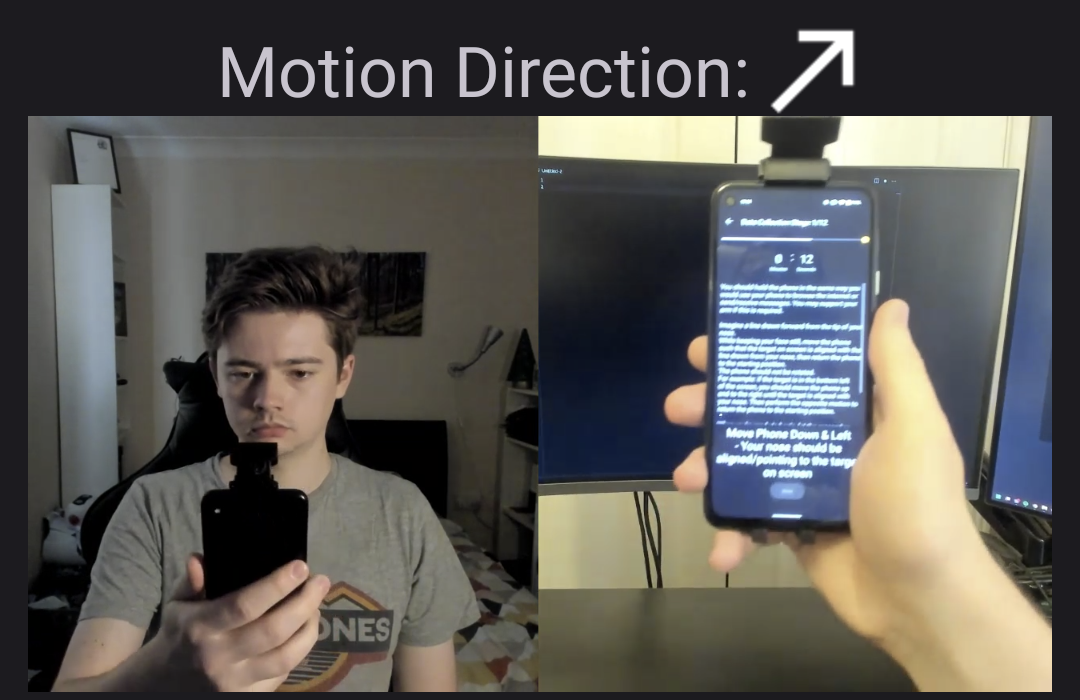
\includegraphics[width=0.5\textwidth]{CountDown_cropped.png}
  \caption{\tempnote{TODO: Replace with Image showing diff between head vs phone moving resulting in similar photo (at least head pose)}}
  \label{fig:teaser}
  \Description{Diagram showing how a the head pose observed by the front-facing camera of a mobile device, caused by the movement of the head, can be replicated by keeping the head still and instead moving the camera.}
\end{teaserfigure}

\maketitle
%% Content Lists %%

% \clearpage
% \restoregeometry
% \newpage

% \setcounter{page}{0}
% \pagenumbering{roman}
% \pagestyle{fancy}

% \tableofcontents
% \clearpage
% \newpage
% \addcontentsline{toc}{section}{\listfigurename}
% \listoffigures
% \clearpage
% \newpage
% \addcontentsline{toc}{section}{\listtablename}
% \listoftables
% \clearpage
% \newpage

% Tell TexCount to start counting words again
%TC:endignore

% Reset Page Styling and numbering for rest of doc
% \setcounter{page}{1}
% \pagenumbering{arabic}
